\documentclass[]{scrartcl}

\usepackage{amsmath}
\usepackage{amssymb}
\usepackage[utf8]{inputenc}
\usepackage[T1]{fontenc}
\usepackage{lmodern}
\usepackage{ngerman}
\usepackage{geometry}
\usepackage{graphicx}
\usepackage{wrapfig}
\usepackage{caption}
\usepackage{wasysym}
\usepackage{siunitx}
\usepackage{picinpar}
\usepackage{tikz}
\usepackage{float}

\renewcommand{\figurename}{Abb.}
\usepackage[
	colorlinks=true,
	urlcolor=blue,
	linkcolor=black
]{hyperref}


%Hier Titel und so
\newcommand{\versuchnummer}{V49} 
\newcommand{\versuchname}{Messung von Diffusionskonstanten mittels gepulster Kernspinresonanz} 
\newcommand{\versuchdatum}{11.01.2016} 


\title{Versuch \versuchnummer\\ \versuchname}
\subtitle{Physikalisches Fortgeschrittenenpraktikum}
\author{Robert Rauter und Björn Lindhauer}
\date{\versuchdatum} 
\begin{document}
\begin{titlepage}
{\large \versuchdatum}
\vspace{7cm}
\begin{center}
\textbf{\huge Versuch \versuchnummer}\\
\vspace{0.5cm}
\textbf{\huge \versuchname}\\
\vspace{0.2cm}
\textbf{ Physikalisches Fortgeschrittenenpraktikum}\\
\vspace{9cm}

{\Large Robert Rauter \ \ \hspace{1.5cm} und \hspace{1.5cm} Björn Lindhauer}\\
{ \url{robert.rauter@tu-dortmund.de} \ \ \hspace{2cm} \url{bjoern.lindhauer@tu-dortmund.de}}
\end{center}
\end{titlepage}
\section{Einleitung}
Die Grundlage der Kernspinresonanz ist, dass sich magnetische Momente der Atomkerne beim wirken eines äußerem Magnetfeld ausrichten. Die Ausrichtung kann durch Einstrahlung von Hochfrequenzquanten mit geeigneter Frequenz verändert werden und so können verschiedene magnetische Eigenschaften einer Probe untersucht werden.\\
Zum einen können Resonanzphänomene beobachtet werden, indem die Energieaufnahme in Abhängigkeit der Frequenz aufgenommen wird. So lassen sich Rückschlüsse auf lokale Magnetfelder anhand der Resonanzstellen schließen. Mit diesen Daten kann die Struktur der Probe rekonstruiert werden.\\
Zum anderen kann der zeitlicher Verlauf von Auf- und Abbau eines Magnetfeldes bestimmt werden. Außerdem lässt sich die Diffusionskonstante einer Probe bestimmen, da sich durch die Diffusion die Anzahl der Momente im Messabschnitt ändert und folglich das statische Magnetfeld der Probe verändert ist. Die Resonanzbedingung ändert sich und aus dieser Änderung lässt sich die Diffusionskonstante bestimmen. Da Resonanzbedingung erfüllt werden sollen, werden Hochfrequenzimpulse benötigt, welches dieser Methode ihren Namen gepulste Kernspinresonanz gab.\\
In diesen Versuch soll mit der gepulsten Kernspinresonanz eine Probe untersucht werden.
\section{Theoretische Grundlagen}
\subsection{Magnetisierung}
Zunächst wird angenommen, dass die Probe im thermischen Gleichgewicht mit der Umgebung steht, da Konvektionsströme nicht Bestandteil der Betrachtungen sind.\\
Des weiteren sei ein homogenes Magnetfeld $B_0\ \vec{e_z}$ angelegt.\\
Durch dieses Feld spalten die entarteten Kernspinzustände
Magnetisierung einer Probe, die im thermischen Gleichgewicht mit der Umgebung steht mit der Spinquantenzahl $I$ in $2I+1$ äquidistante Unterniveaus auf, welche den Abstand $\Delta E = \gamma B_0 \hbar$ besitzen.\\
Die Besetzung der Niveaus erfolgt nach der Boltzmann-Verteilung. Es folgt daraus das Besetzungszahlverhältnis 
\begin{align}
\frac{N\left(m\right)}{N\left(m-1\right)}=\exp \left(-\frac{\gamma B_0\hbar}{k_\text{B}T}\right)
\end{align}
bei gegebenen $T$.\\
Da die Besetzung folglich nicht homogen über alle Zustände ist, besitzt der Kern eine Kernspinpolarisation
\begin{align}
\left\langle I_Z \right\rangle = \frac{\sum\limits_{m=-I}^{I} \hbar m \exp\left(-\beta m\gamma B_0 \hbar \right)}{\sum\limits_{m=-I}^{I} \exp\left(-\beta m\gamma B_0 \hbar \right)} \label{eq_izallgemein}\hspace*{0.5cm}\text{.}
\end{align}
Im folgenden werden nur noch Protonen betrachtet, es ist somit $I=\frac{1}{2}$. Ein Niveau spaltet sich in zwei Unterniveaus auf mit den Quantenzahlen $m=-\frac{1}{2}$ und $m=+\frac{1}{2}$. Abbildung \ref{fig_aufspaltung} veranschaulicht dies.
\begin{figure}[H]
\centering
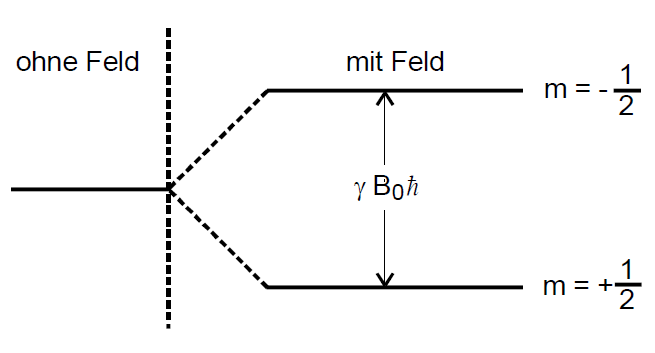
\includegraphics[width=8cm]{images/aufspaltung_magnetfeld.png}
\caption{Toller Titel (1)}
\label{fig_aufspaltung}
\end{figure}
Für die Exponentialfunktion in \ref{eq_izallgemein} kann eine lineare Näherung eingesetzt werden, falls
\begin{align}
m\gamma B_0 \hbar \ll k_\text{B}T 
\end{align}
ist, welches für Magnetfelder in der Größenordnung von 1 Tesla und Temperaturen nahe der Zimmertemperatur gegeben ist.\\
Es ergibt sich
\begin{align}
\left\langle I_Z \right\rangle_{\text{P}}= -\frac{\hbar^2}{4}\frac{\gamma B_0}{k_\text{B}T}\hspace*{0.5cm}\text{.} \label{eq_iznahrung}
\end{align}
Da die Kernspinpolarisation im direkten Zusammenhang mit den magnetischen Momenten $\vec{\mu}_I$ stehen, ist eine makroskopische Magnetisierung $\vec{M_0}$ der Probe messbar, die durch die Summe aller Einzelmomente pro Volumen
\begin{align}
\vec{M_0}=\sum\limits_{i}^{}\frac{\mu_0\vec{\mu}_i}{V}
\end{align}
gegeben ist.\\
Es ist
\begin{align}
\left\langle \vec{M_0}_z \right\rangle =N\gamma \mu_0 \left\langle I_Z \right\rangle_{\text{P}} :=\left\langle M_0 \right\rangle\hspace*{0.5cm}\text{.}
\end{align}
Wird nun \ref{eq_iznahrung} eingesetzt, so ergibt sich
\begin{align}
\left\langle M_0 \right\rangle = N\frac{\hbar^2}{4}\mu_0\frac{\gamma^2 B_0}{k_\text{B}T}:=M_0
\end{align}
als Gleichgewichtsmagnetisierung bei Temperatur $T$.
\subsection{Larmor-Präzession}
-$\vec{M}$ wird aus Gleichgewichtslage $\vec{M_0}$ durch Hochfrequenzquanten mit Energie $\Delta E$ gebracht
-Magnetisierung durch viele Spins --> klassische Betrachtung
-Drehmoment
\begin{align}
\vec{D}=\vec{M}\times B_0 \vec{e_z}
\end{align}
-über Kreiselgleichung lässt sich herleiten
\begin{align}
\frac{d \vec{M}}{d t} = \gamma \vec{M}\times B_0 \vec{e_z}
\end{align}
- Lösung der DGL Komponentenweise
\begin{align}
M_x= 0 \\
M_y= A \cos \gamma B_0 t \\
M_z= -A \sin \gamma B_0 t
\end{align}
--> Präzession um  $\vec{e_z}$-Achse mit der Larmor-Frequenz genannten
\begin{align}
\omega_L =\gamma B_0
\end{align}
\subsection{Relaxationserscheinungen}
\section{Durchführung}

\section{Auswertung}

\subsection{Messung der Relaxationszeit T$_1$}
Die z-Komponente der Magnetisierung weist einen exponentiellen Zusammenhang mit dem Zeitabstand $\tau$ zwischen den 90$^{\circ}$ auf, wie in Formel \ref{eq_T1} dargestellt ist. \\
\begin{align}
M_{z}(\tau)=M_0(1-2\exp(-\tau/T_1))
\label{eq_T1}
\end{align}
Zur Bestimmung von T$_1$ wird eine nicht-lineare Ausgleichsrechnung mit den in Tabelle \ref{tab_t1} angegebenen Messwerten durchgeführt. \\
\begin{center}
	\begin{tabular}{|c|c||c|c|}
		\hline	$\tau$ [s]	&	M$_z$ [V] & $\tau$ [s]	&	M$_z$ [V]\\
		\hline	0,003	&	1,47	&	1,503	&	-0,09	\\
		\hline	0,013	&	1,43	&	1,603	&	-0,12	\\
		\hline	0,023	&	1,41	&	1,703	&	-0,18	\\
		\hline	0,043	&	1,39	&	1,803	&	-0,24	\\
		\hline	0,063	&	1,37	&	1,903	&	-0,29	\\
		\hline	0,083	&	1,35	&	2,003	&	-0,3	\\
		\hline	0,103	&	1,31	&	2,203	&	-0,47	\\
		\hline	0,153	&	1,27	&	2,403	&	-0,58	\\
		\hline	0,203	&	1,21	&	2,603	&	-0,67	\\
		\hline	0,253	&	1,17	&	2,803	&	-0,75	\\
		\hline	0,303	&	1,13	&	3,003	&	-0,82	\\
		\hline	0,353	&	1,07	&	3,203	&	-0,9	\\
		\hline	0,403	&	1,01	&	3,403	&	-0,95	\\
		\hline	0,503	&	0,91	&	3,603	&	-1,01	\\
		\hline	0,603	&	0,81	&	3,803	&	-1,06	\\
		\hline	0,703	&	0,68	&	4,003	&	-1,1	\\
		\hline	0,803	&	0,58	&	4,503	&	-1,2	\\
		\hline	0,903	&	0,48	&	5,003	&	-1,28	\\
		\hline	1,003	&	0,38	&	5,503	&	-1,33	\\
		\hline	1,103	&	0,3	&	6,003	&	-1,34	\\
		\hline	1,203	&	0,2	&	7,003	&	-1,42	\\
		\hline	1,303	&	0,12	&	8,003	&	-1,44	\\
		\hline	1,403	&	0,04	&	9,003	&	-1,47	\\
		\hline
	\end{tabular}
	\captionof{table}{Aufgenommene Messwerte der z-Komponente der Magnetisierung in Abhängigkeit vom Zeitabstand $\tau$ zwischen den 90$^{\circ}$-Pulsen.}
	\label{tab_t1}
\end{center}
Mit Gleichung \ref{eq_T1} ergibt eine nicht-lineare Ausgleichsrechnung mit Python folgende Fitparameter:

		
\section{Quellen}

\end{document}